\chapter{Notation overview}\label{ch:appendix_notation}
This chapter presents listing of the mathematical notation used in this thesis:

\bigskip
\begin{tabular}{ll}
	$X$ & Capital letter denotes a random variable.\\
	&\\
	$x$ & Lowercase letter denotes a concrete instantiation of the variable $X$.\\
	&\\
	$\vars{X}$ & Capital bold letter denotes a set of random variables.\\
	&\\
	$\vars{x}$ & Lowercase bold letter denotes an instantiation of all variables in the set $\vars{X}$.\\
	&\\
	$val(\vars{X})$ & Set of all possible instantiations of variables $\vars{X}$.\\
	&\\
	$Parents(X)$ & Set of parent variables of variable $X$ in a Bayesian network.\\
	&\\
	$parents(X)$ & Instantiation of parent variables of variable $X$ in a Bayesian network.\\
	&\\
	$Children(X)$ & Set of child variables of variable $X$ in a Bayesian network.\\
	&\\
	$children(X)$ & Instantiation of child variables of variable $X$ in a Bayesian network.\\
	&\\
	$N_x$ & Number of samples of a dataset for which variable $X$ has the value $x$.\\
	&\\
	$N_{x,\vars{pa}}$ & Number of samples of a dataset for which $X$ has the value $x$ and variables\\
	                  & $Parents(X)$ have the value $\vars{pa}$.\\
	&\\
	$\sum_\vars{X} (\dots)$ & Summation over instantiations $\vars{x}$ of the variables $\vars{X}$.\\
	&\\
	$P(\vars{X})$ & Probability distribution over variables $\vars{X}$.\\
	&\\
	$P(\vars{x})$ & Probability of variables $\vars{X}$ having the concrete instantiation $\vars{x}$.\\
\end{tabular}










\chapter{CD Content}\label{ch:appendix_cd_content}
Content of the enclosed CD is organized into the following directories:
\begin{itemize}
    \item \srccode{1-benchmarks/}: Network \srccode{.net} files, datasets and measurements related to the first practical application.
    \item \srccode{2-crime/}: Vector images of the final three networks that resulted from the analysis of criminality. Also contains the original dataset, its discretized version, networks learnt during the feature elimination process and records of analysis of the crime impact factor.
    \item \srccode{3-spam/}: Datasets (the original dataset, its discretized version, train and test sets for holdout testing and for 5-fold cross-validation). Also contains measurement records and figures.
    \item \srccode{program/}: Program source codes compilable using the \emph{ant} build tool and also runnable compiled version in \srccode{program/bin-precompiled}.
    \item \srccode{text/}:  Electronic version of this thesis and {\LaTeX} sources, including all figures.
\end{itemize} 





\chapter{Crime analysis\,--\,final networks}\label{ch:appendix_crime_net}
This chapter contains the three networks that are result of the crime analysis performed in Section~\ref{ch:practical_crime}. Because of their size, each network is on its own A3 page. If you have trouble reading variable names in the printed version please see the electronic version of this thesis or the original figures on the encolsed CD within the directory \srccode{2-crime/final networks/}.


\begin{hugepage}
\pdfpagewidth=2\pdfpagewidth
\begin{figure}[h]
    \centering
    \vspace*{-2.5cm}
    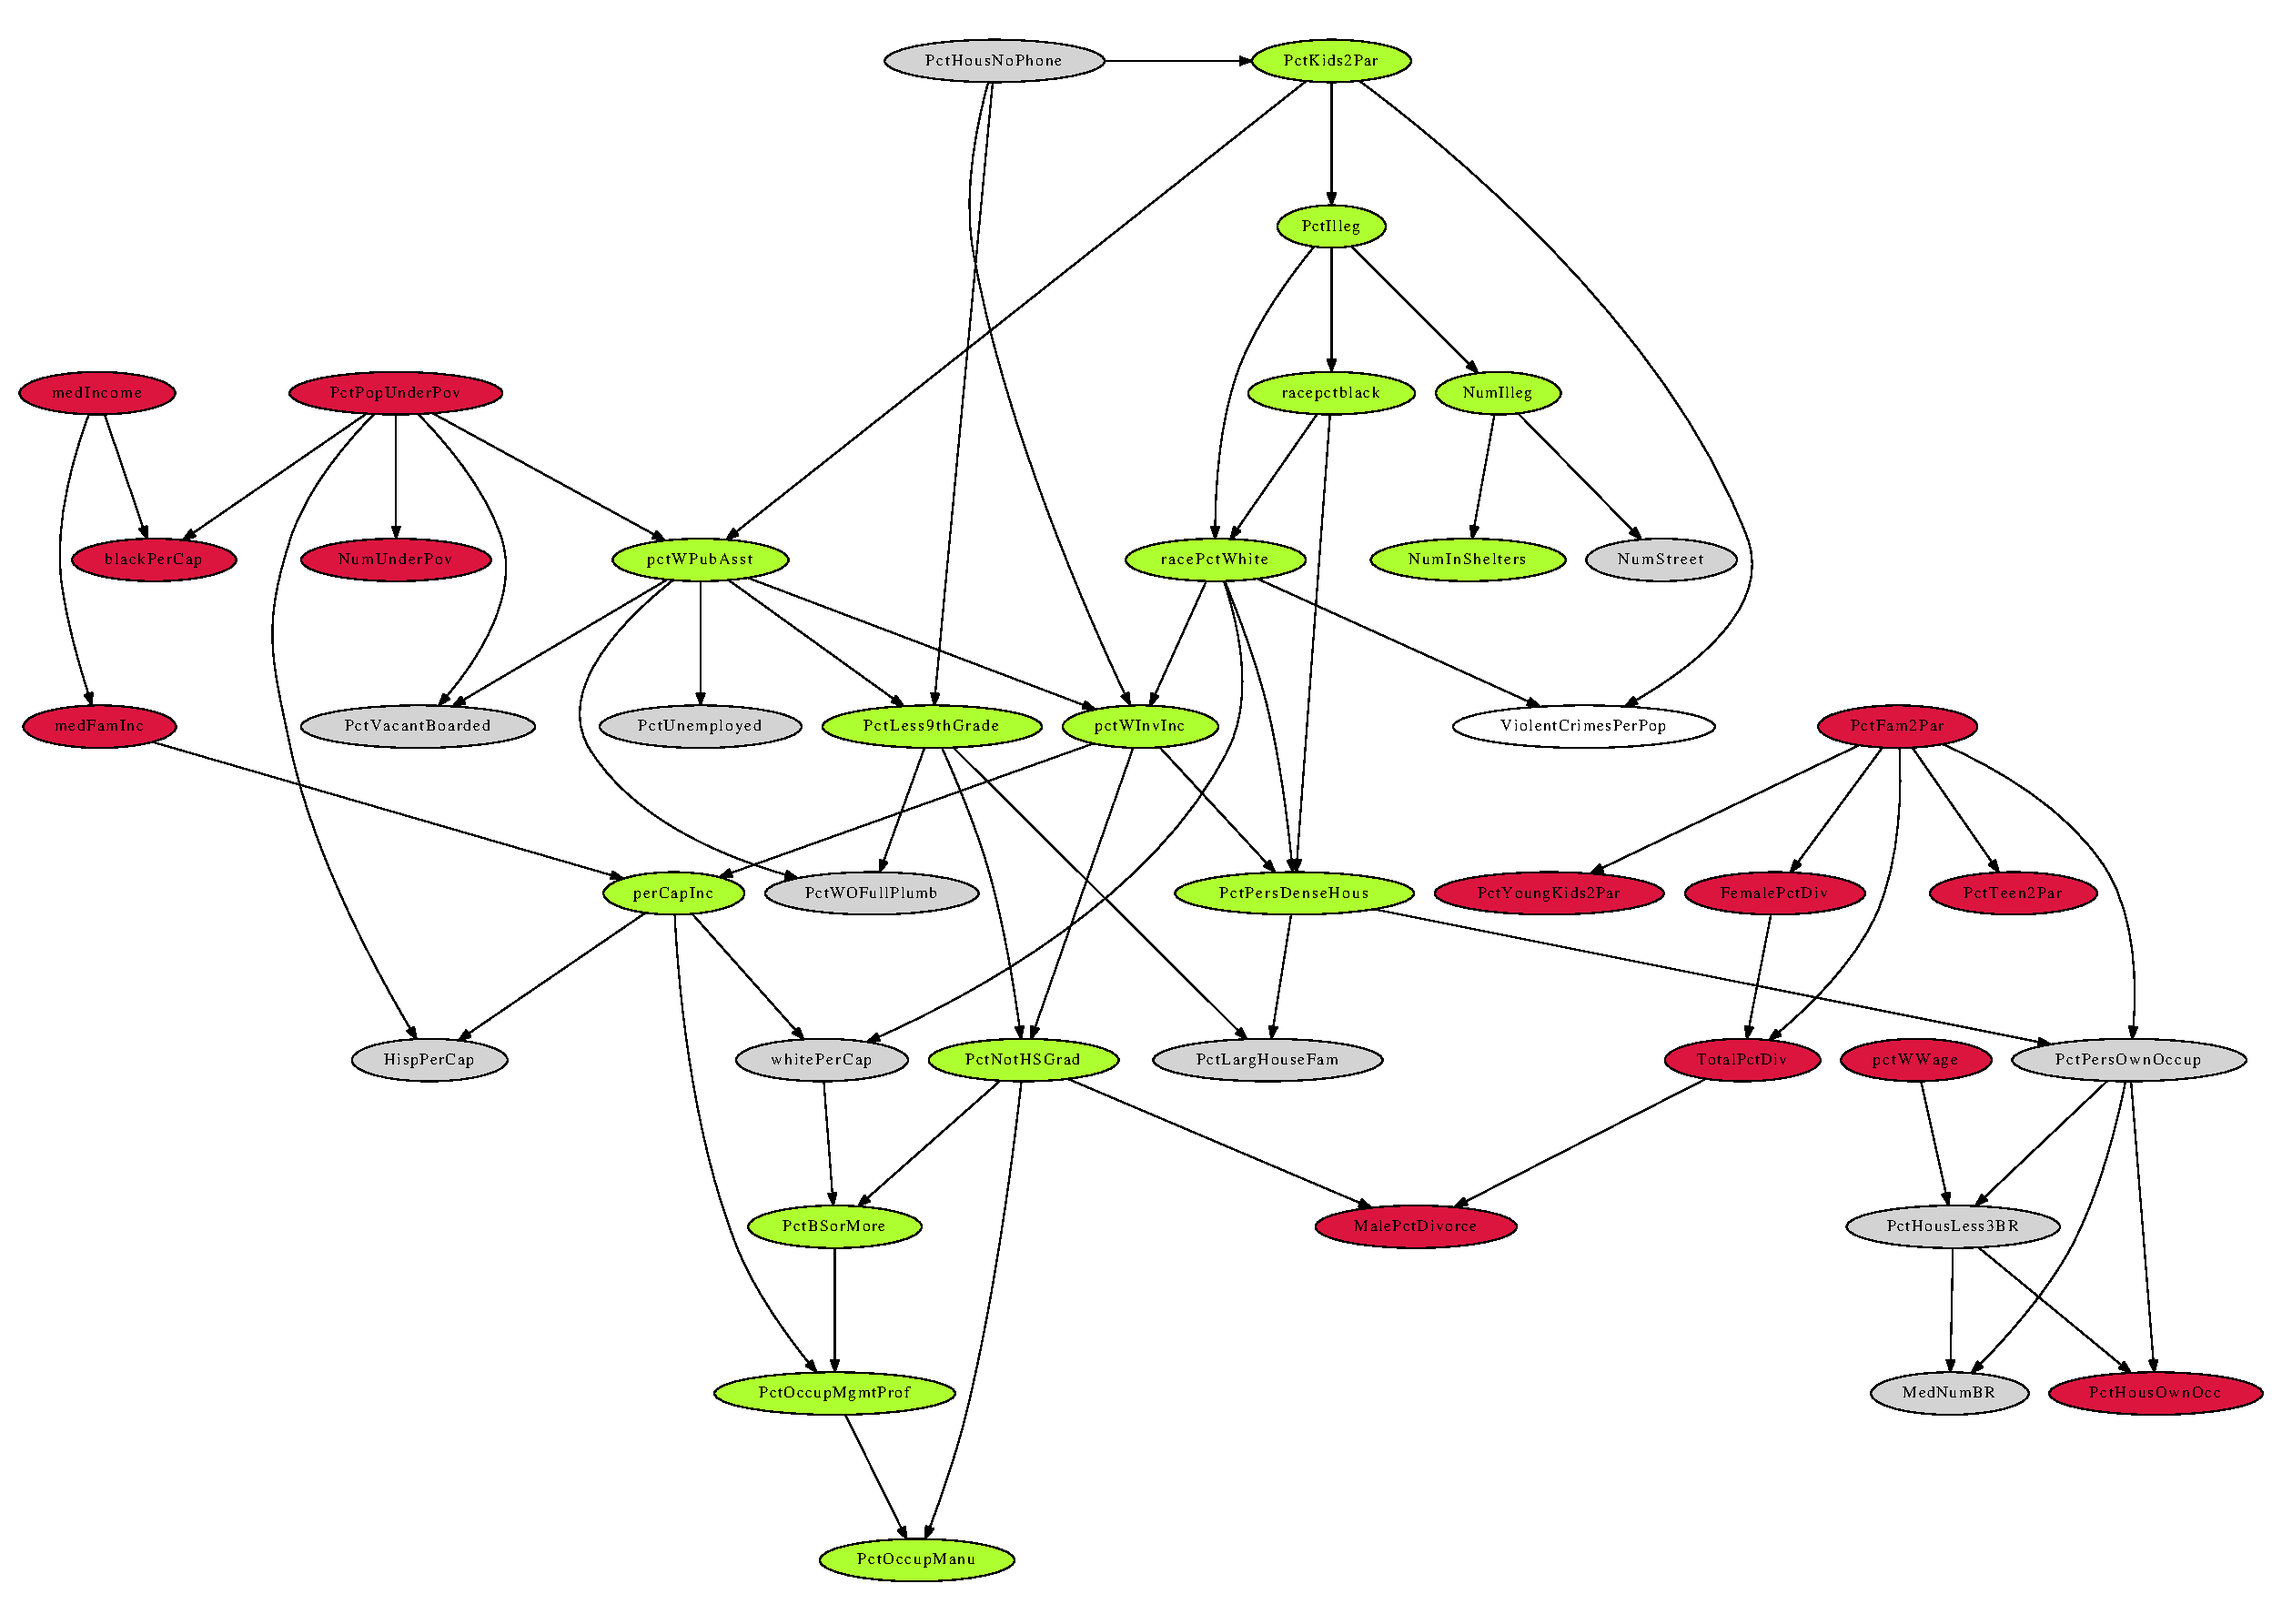
\includegraphics[scale=0.834]{fig/top-40_intersection_tolerance-1}
    \caption{Bayesian network for crime containing top 40 attributes with the highest crime impact factor.
    \\Legend: Green variables influence the $ViolentCrimesPerPop$ the same way as in the network with all 100 features. Influence of red variables is significantly different and therefore these variables shouldn't be considered.}
    \label{fig:crime_net_top40}
\end{figure}
\end{hugepage}

\begin{hugepage}
\pdfpagewidth=2\pdfpagewidth
\begin{figure}[h]
    \centering
    \vspace*{-2.5cm}
    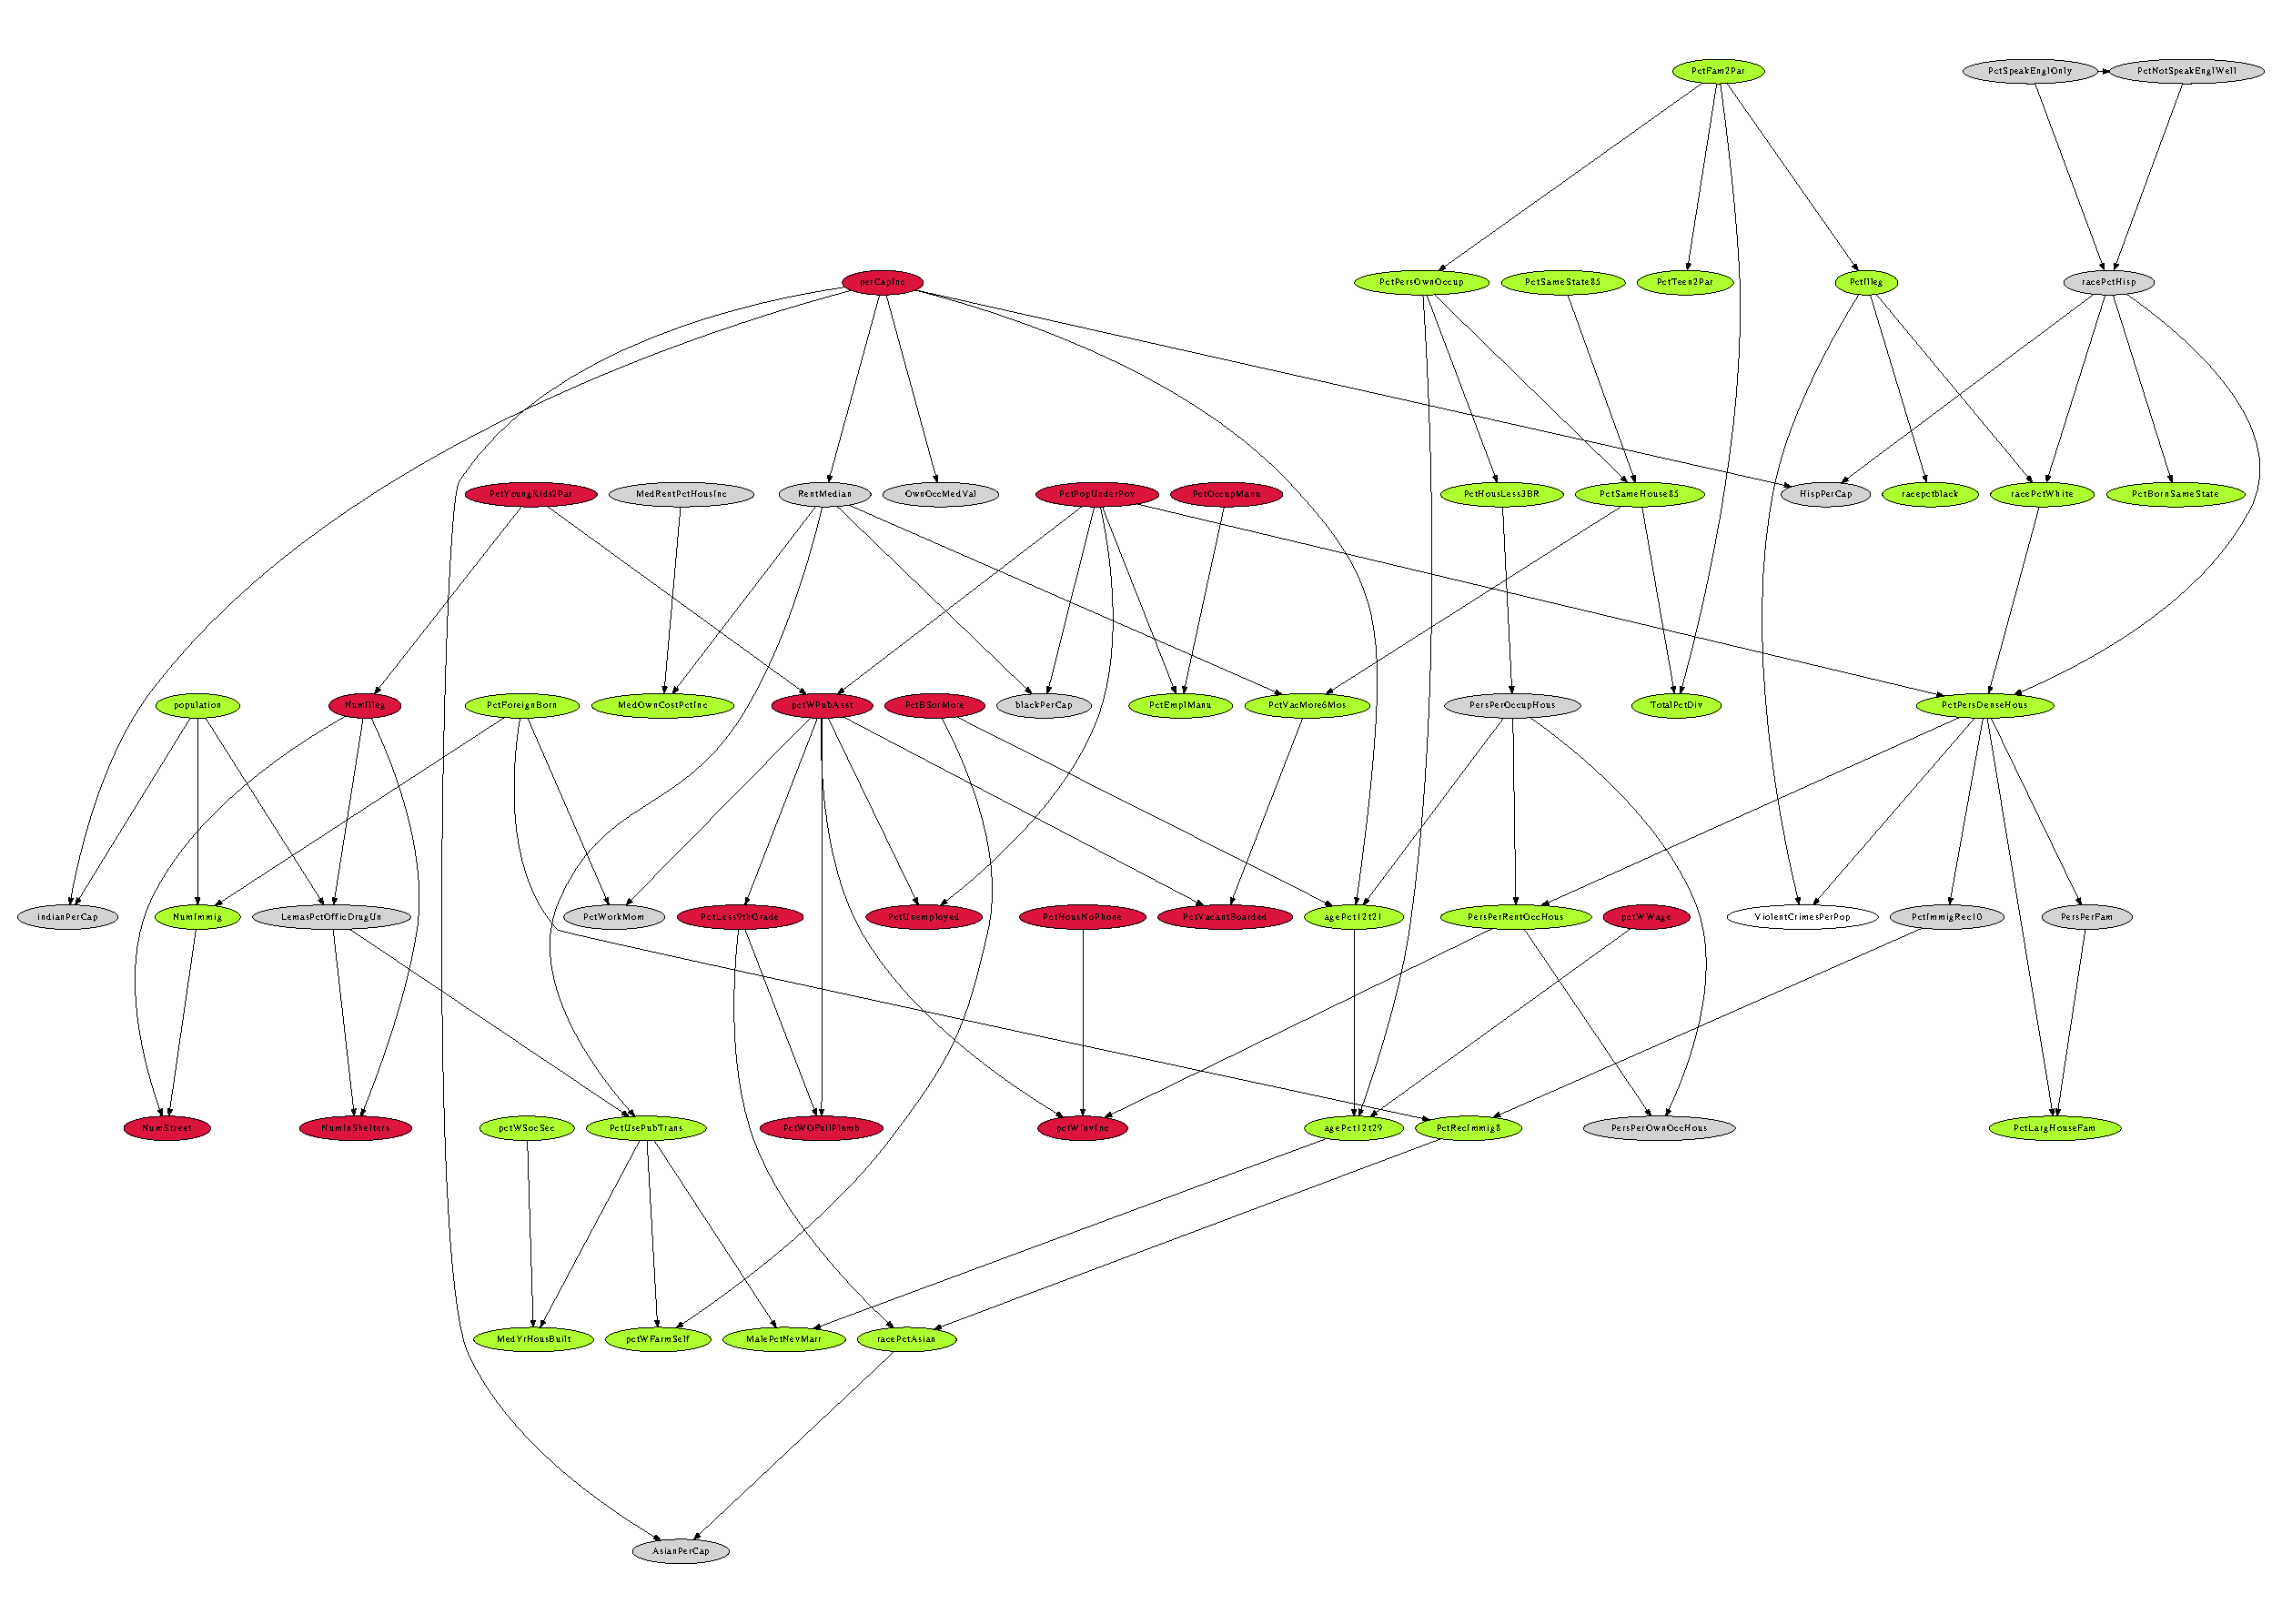
\includegraphics[scale=0.83]{fig/round-3_intersection_tolerance-1}
    \caption{Final Bayesian network for crime after three rounds of iterative elimination of similar variables.
    \\Legend: Green variables influence the $ViolentCrimesPerPop$ the same way as in the network with all 100 features. Influence of red variables is significantly different and therefore these variables shouldn't be considered.}
    \label{fig:crime_net_round3}
\end{figure}
\end{hugepage}

\begin{hugepage}
\pdfpagewidth=2\pdfpagewidth
\begin{figure}[h]
    \centering
    \vspace*{-2.5cm}
    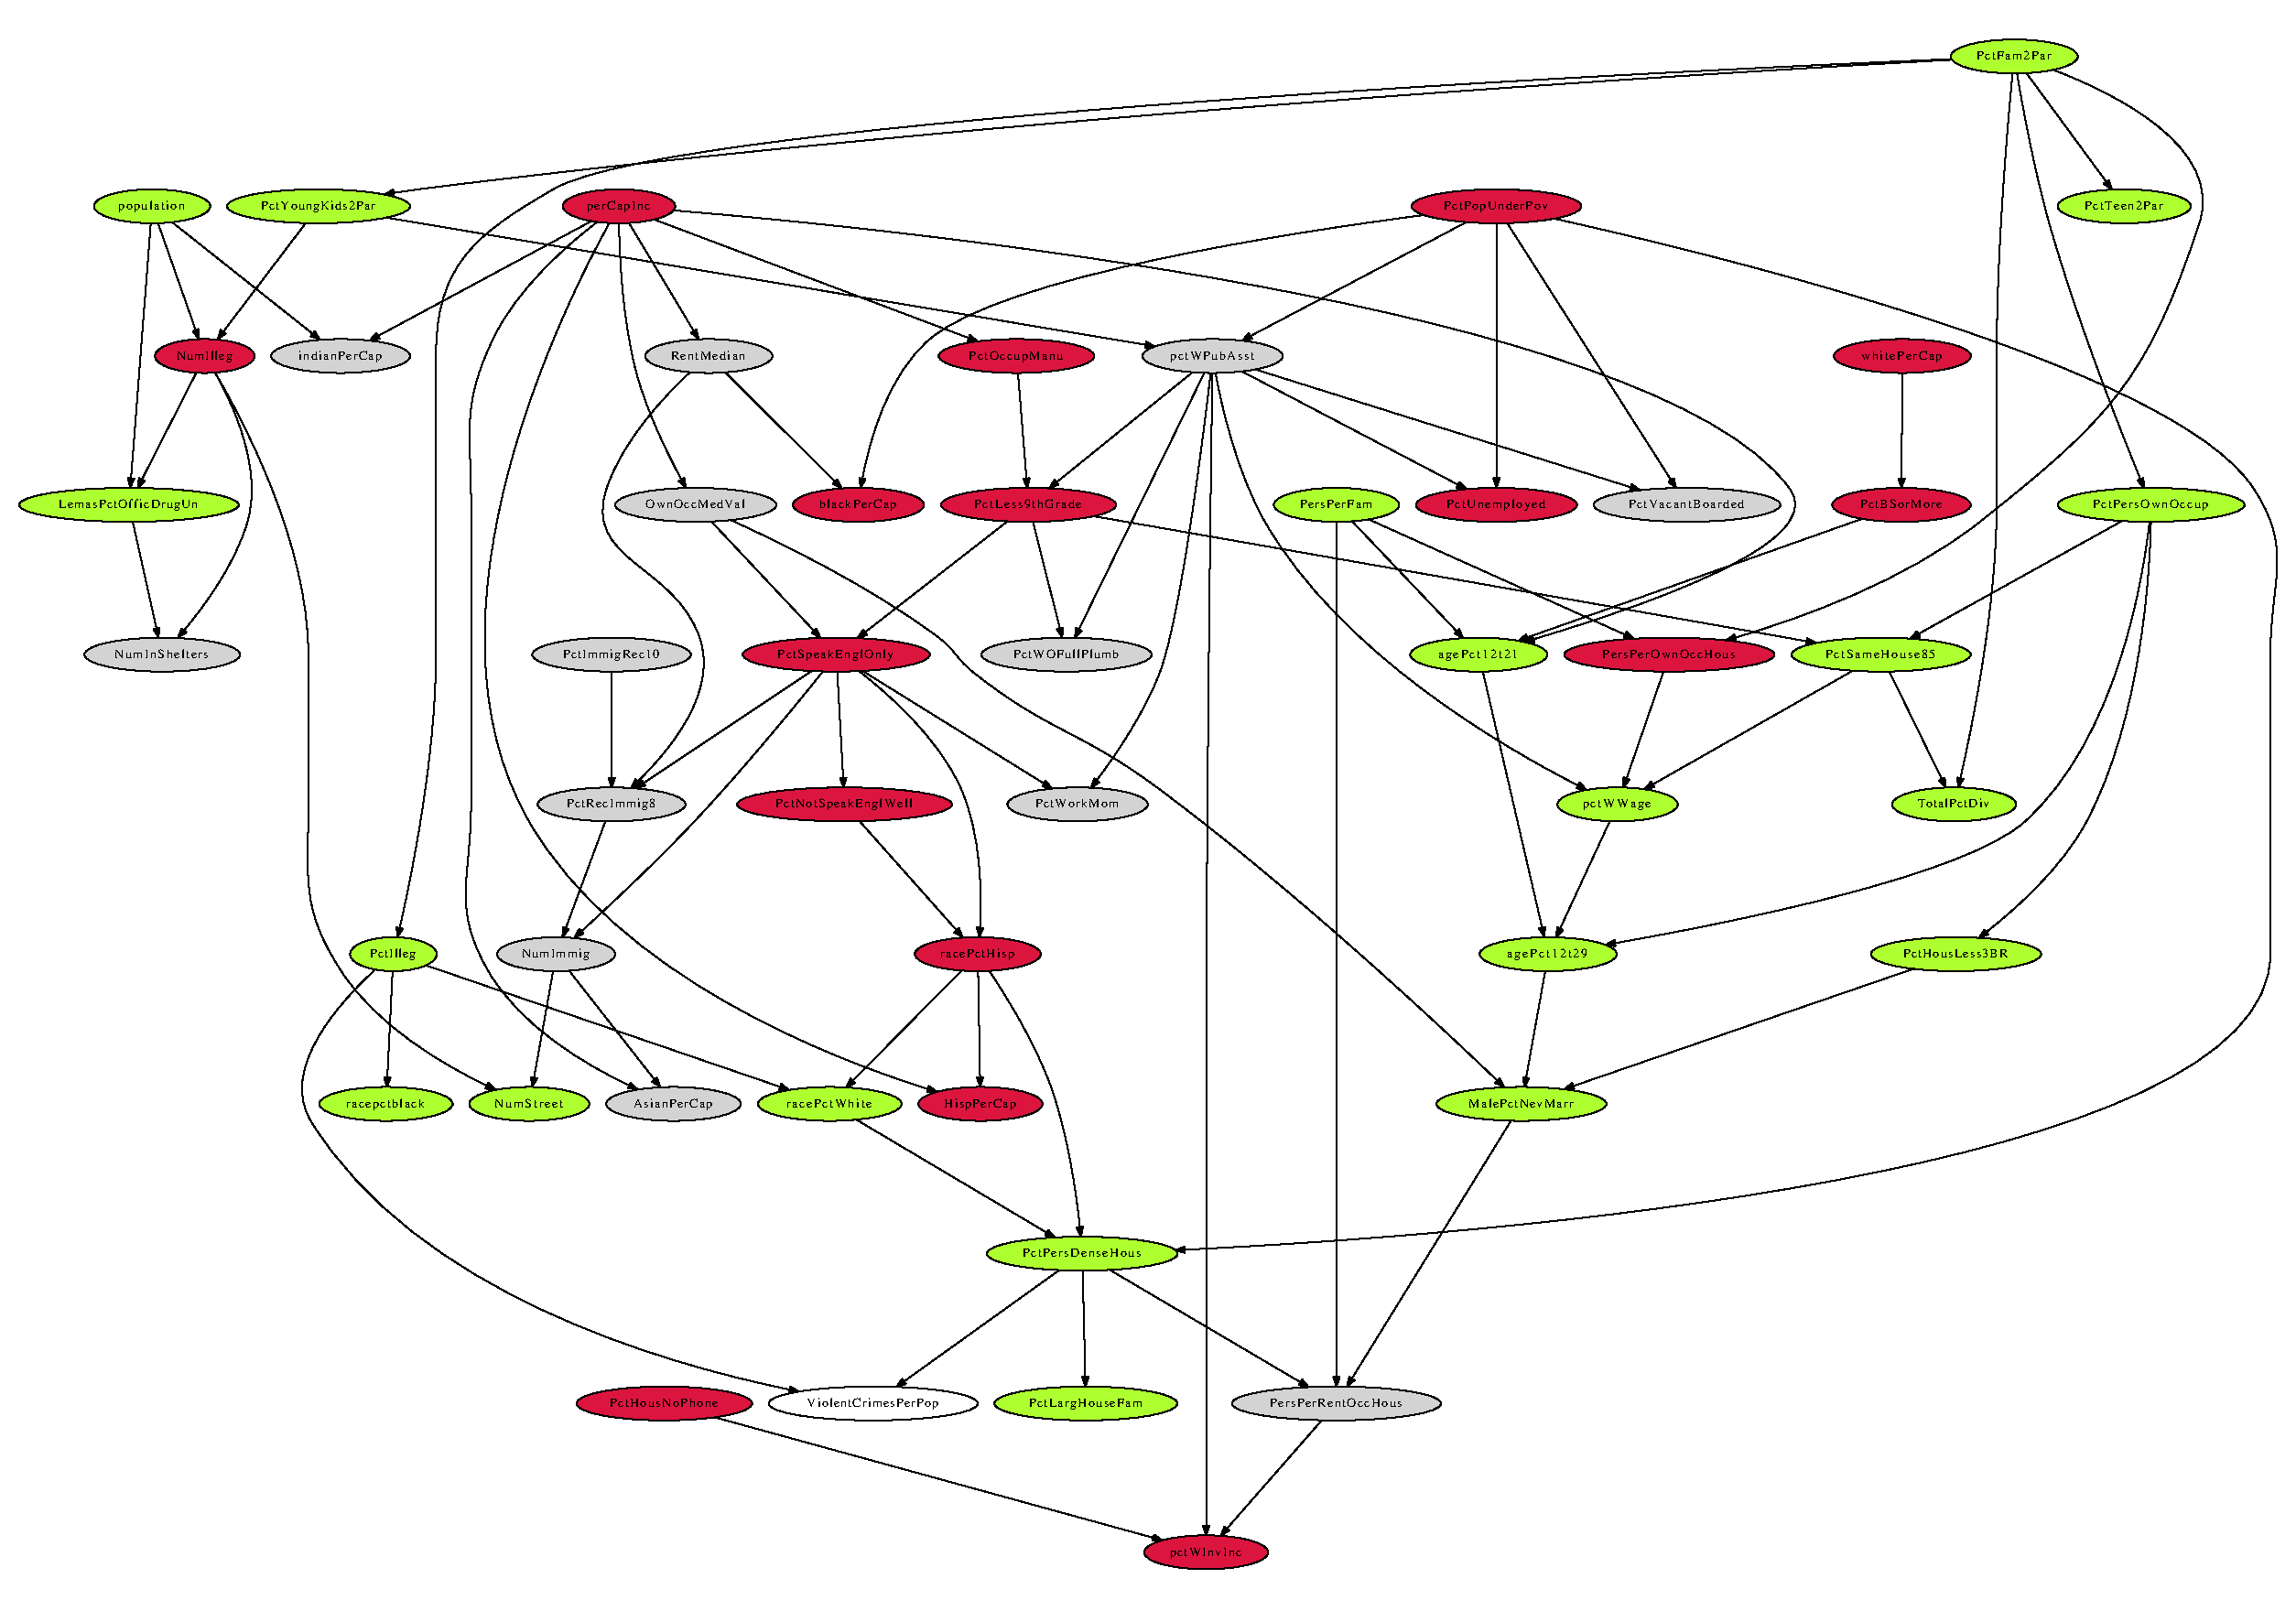
\includegraphics[scale=0.83]{fig/round-4_intersection_tolerance-1}
    \caption{Final Bayesian network for crime after three rounds of iterative elimination of similar variables and additional removal of variables whose crime impact factor is less than 0.07.
    \\Legend: Green variables influence the $ViolentCrimesPerPop$ the same way as in the network with all 100 features. Influence of red variables is significantly different and therefore these variables shouldn't be considered.}
    \label{fig:crime_net_round4}
\end{figure}
\end{hugepage}


